\documentclass{beamer}
\usepackage[ngerman]{babel}
\usepackage[T1]{fontenc}
\usepackage[utf8x]{inputenc}

%\setbeameroption{show notes on second screen=left}
%\setbeameroption{show notes on second screen}
%\usetheme{default}
%\useoutertheme{smoothbars} %overview at top
\useinnertheme[shadow=true]{rounded} %grey preview of bullet points
%\beamersetuncovermixins{\opaqueness<1>{25}}{\opaqueness<2->{15}}
\beamertemplatenavigationsymbolsempty %remove navigation symbols

\usepackage{tikz}
\usetikzlibrary{arrows}
\tikzstyle{block} = [draw,fill=blue!20,minimum size=2em]
\tikzstyle{block2} = [draw,fill=red!20,minimum size=2em]
\tikzstyle{block3} = [draw,fill=white,minimum size=2em]

\usepackage{ifthen}
\usepackage{graphicx}
\usepackage{listings}
\usepackage{cancel}
\def \korrekturfarbe {blue}
\renewcommand{\CancelColor}{\color{\korrekturfarbe}}

\title{Übungsblatt 1}
\subtitle{Algorithm Engineering}
\author{Waldemar Smirnow, Michael Stypa}
\institute{Universität Osnabrück}
\date{\today}

\begin{document}
\begin{frame}
    \titlepage
\end{frame}

%queue
%-first-in-first-out data structure
%-first-come-first-server processing of a queue
%-performs the function of a buffer
%-doesnt have a capacity
%-can be empty
%-queue underflow
%-queue overflow

%klassischen internen Implementierungen des Datentyps Stack besprochen
\section{Aufgabe 1.1a}
\begin{frame}
  \frametitle{Queue}
  \framesubtitle{Die Datenstruktur}
  \begin{itemize}
    \item Warteschlange / Puffer
    \item FIFO (first-in-first-out)
    \item Nimmt beliebig viele Objekte auf
  \end{itemize}
\end{frame}

\begin{frame}
  \frametitle{Queue}
  \framesubtitle{Im Beispiel}
  \begin{figure}
    \centering
    \begin{tikzpicture}
      \uncover<1-2>{\node[block] at (-1,0) (item1) {$1$};}
      \foreach \y [evaluate=\y as \x using \y-1] in {2,3,4,5} {
        \node[block] at (-\y,0) (item\y) {$\y$};
      }
      \uncover<2>{\node[block,fill=green!20] at (-6,0) (item6) {$v$};}
      \uncover<3->{\node[block] at (-6,0) (item6) {$v$};}
      \uncover<3->{\node[block,fill=green!20] at (-1,2) (item1) {$1$};}
    \end{tikzpicture}
  \end{figure}
  \begin{itemize}
    \item<2-> enqueue(type $v$) Hängt $v$ an den Anfang der Queue an
    \item<3-> type dequeue() Liefert ältestes Element der Queue und entfernt es
  \end{itemize}
\end{frame}

\begin{frame}
  \frametitle{Queue}
  \framesubtitle{Implementierungen (optimal im RAM-Modell)}
  Array + Zeiger auf oberstes Element + Zeiger auf unterstes Element
  \begin{figure}
    \centering
    \begin{tikzpicture}[>=latex']
      \foreach \y in {1,2,3,4,5} {
        \node[block] at (3*\y/4,0) (item\y) {$\y$};
      }
      \draw[<-] (item1.north) -- +(0,0.5);
      \draw[<-] (item5.south) -- +(0,-0.5);
    \end{tikzpicture}
  \end{figure}

  Zeigerverkettete Liste + Zeiger auf oberstes Element + Zeiger auf unterstes Element
  \begin{figure}
    \centering
    \begin{tikzpicture}[>=latex']
      \foreach \y in {1,2,3,4,5} {
        \node[block] at (-\y,0) (item\y) {$\y$};
        \draw[->] (item\y.west) -- +(-0.25,0);
      }
      \draw[<-] (item5.north) -- +(0,0.5);
      \draw[<-] (item1.south) -- +(0,-0.5);
    \end{tikzpicture}
  \end{figure}
\end{frame}

%ihr Verhalten im Externspeicher-Setting analysiert
\begin{frame}
  \frametitle{Queue}
  \framesubtitle{Verhalten im Externspeicher-Setting}
  $B=3$
  \begin{figure}
    \centering
    \begin{tikzpicture}[>=latex']
      \foreach \y in {4,5,6} {
        \node[block] at (3*\y/4,0) (item\y) {$\y$};
      }
      \node (d1) [below of=item5] {intern};
    \end{tikzpicture}
    \hspace{10mm}
    \begin{tikzpicture}[>=latex']
      \foreach \y in {1,2,3} {
        \node[block2] at (3*\y/4,0) (item\y) {$\y$};
      }
      \node (d1) [below of=item2] {extern};
    \end{tikzpicture}
  \end{figure}
  Anzahl der I/Os (für beliebige Abfolge von Operationen)
  \begin{itemize}
    \item $O(1)$ pro Operation
  \end{itemize}
\end{frame}

%eine Modifikation vorgeschlagen, die in diesem Setting beweisbar besser funktioniert
\begin{frame}
  \frametitle{Extern-Queue}
  \framesubtitle{}
  \begin{itemize}[<+->]
    \item Interner Speicher ("Puffer"): Array $J$ der Größe $2B$; restliche Daten extern
    \item $J$ enthält zu jedem Zeitpunkt die zwei Blöcke mit Anfang und Ende der Queue
  \end{itemize}

  enqueue(type $v$)
  \begin{itemize}[<+->]
    \item Falls Anfang-Block Platz hat: Füge $v$ ein. \bf{Kein I/O}
    \item Falls Anfang-Block voll: Vollen Anfang-Block auslagern und neuen im internen Speicher anfangen. \bf{1 I/O}
  \end{itemize}

  type dequeue($v$)
  \begin{itemize}[<+->]
    \item Falls Ende-Block mehr als einen Eintrag hat: $v$ ausliefern und aus dem Block löschen. \bf{Kein I/O}
    \item Falls Ende-Block einen Eintrag hat: Eintrag ausliefern und neuen Ende-Block laden. \bf{1 I/O}
  \end{itemize}
\end{frame}


\section{Aufgabe 1.1b}
\begin{frame}{Aufgabe 1.1 (b)}

  Betrachte den Algorithmus \emph{Counting Sort} zum Sortieren von $N$ vielen Zahlen aus dem Universum $\{1,2,\dots{},k\}$ in linearer Zeit $O(N+k)$. 
  Sei $k = \alpha \cdot M$.
  Wieviele I/O-Operationen benötigt der Algorithmus, falls $\alpha = 0,5$ bzw. falls $\alpha > 1$.
  Kann man den Algorithmus für letzteren Fall einfach verbessern?
\end{frame}

\begin{frame}{Counting Sort Algorithmus}
  \begin{itemize}
    \item Zählalgorithmus
    \item Nebenbedingung:
    \begin{itemize}
      \item zu sortierende Elemente sind Integer,
      \item in dem Intervall $[0,k]$
    \end{itemize}
    \item Bestimmt für jedes Eingabeelement die Anzahl der Elemente, die kleiner sind
    \begin{itemize}
      \item Daraus ergibt sich die Position im Ausgabearray
    \end{itemize}
    \item Laufzeit $O(n+k)$
    \item Einsatz in anderen Sortieralgorithmen (Bsp. Radix Sort)
  \end{itemize}
\end{frame}

\begin{frame}{Counting Sort Algorithmus}
  \begin{itemize}
    \item Speichergrößen
    \begin{itemize}
        \item Eingabearray $A[1\dots n]$
        \item Ausgabearray $B[1\dots n]$
        \item Hilfsarray $C[0\dots k]$
    \end{itemize}
  \end{itemize}
\end{frame}

\begin{frame}{Counting Sort Algorithmus}
  \begin{figure}[htb]
    \centering
    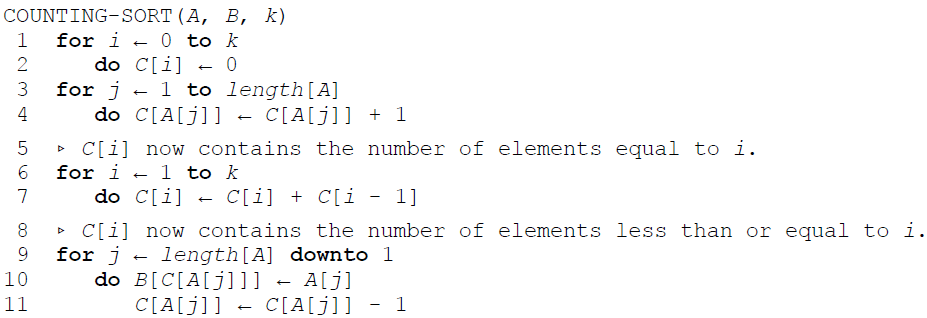
\includegraphics[width=1.1\textwidth]{img/counting-sort}
    \caption{Counting Sort Algorithmus \cite{CormenLeisersonRivestStein200107}} % Seite 148
  \end{figure}
\end{frame}

\begin{frame}{Nachtrag}
  \begin{center}
    Alle {\color{\korrekturfarbe}blau} durchgestrichenen Passagen sind Korrekturen aus der Übung
  \end{center}
\end{frame}

\begin{frame}{Counting Sort Algorithmus}

  \begin{itemize}
    \item[Z. 1-2] Block 1:
    \begin{itemize}
      \item Initialisierung des Hilfsarrays der Größe $k+1$
      \item Anzahl I/O-Operationen:
            \[
              \frac{k+1}{Blockgr.} \Rightarrow O(\xcancel{\frac{k}{Blockgr.}}) \Rightarrow O(k)
            \]
    \end{itemize}
  \end{itemize}
  \vspace{1cm}
  \begin{figure}
    \flushright
    \fbox{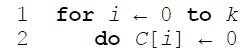
\includegraphics[width=.4\textwidth]{img/counting-sort-b1}}
  \end{figure}
\end{frame}

\begin{frame}{Counting Sort Algorithmus}
  \begin{itemize}
    \item[Z. 3-4] Block 2:
    \begin{itemize}
      \item Zählung der Werte
      \item Inkrementiere $C[A[j]]$ um 1
      \item Anzahl I/O-Operationen:
            \[
              \frac{n}{Blockgr.} + n \Rightarrow O(\xcancel{\frac{n}{Blockgr.} +} n) ~
              \Rightarrow O(n)
            \]
    \end{itemize}
  \end{itemize}
  \vspace{1cm}
  \begin{figure}
    \flushright
    \fbox{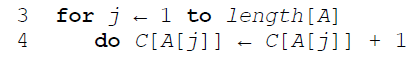
\includegraphics[width=.7\textwidth]{img/counting-sort-b2}}
  \end{figure}
\end{frame}

\begin{frame}{Counting Sort Algorithmus}
  \begin{itemize}
    \item[Z. 6-7] Block 3:
    \begin{itemize}
      \item Berechnung der Ausgabeadressen (Index im Ausgabearray)
      \item Anzahl I/O-Operationen:
            \[
              \frac{k}{Blockgr.} \Rightarrow
              O(\xcancel{\frac{k}{Blockgr.}}) ~
              \Rightarrow O(k)
            \]
    \end{itemize}
  \end{itemize}
  \vspace{1cm}
  \begin{figure}
    \flushright
    \fbox{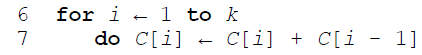
\includegraphics[width=.7\textwidth]{img/counting-sort-b3}}
  \end{figure}
\end{frame}

\begin{frame}{Counting Sort Algorithmus}
  \begin{itemize}
    \item[Z. 9-11] Block 4:
    \begin{itemize}
      \item Kopiere die Werte aus dem Eingabearray in das Ausgabearray,
      \item die Position im Ausgabearray ist $C[A[j]]$
      \item Dekrementiere $C[A[j]]$ um 1
      \item Anzahl I/O-Operationen:
            \[
              \frac{n}{Blockgr.} + 2n \Rightarrow
              O(\xcancel{n + \frac{n}{Blockgr.}}) ~
              \Rightarrow O(n)
            \]
    \end{itemize}
  \end{itemize}

  \begin{figure}
    \flushright
    \fbox{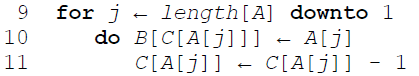
\includegraphics[width=.7\textwidth]{img/counting-sort-b4}}
  \end{figure}
\end{frame}

\begin{frame}{Counting Sort Algorithmus}
  \begin{itemize}
    \item Gesamt Anzahl I/O-Operationen:
    \begin{equation*}
      \frac{k+1}{Blockgr.} +
      \frac{n}{Blockgr.} + n +
      \frac{k}{Blockgr.} +
      \frac{n}{Blockgr.} + 2n =
    \end{equation*}
    \begin{equation*}
      \frac{2(n+k)+1}{Blockgr.}+3n
    \end{equation*}
    \begin{equation*}
      \Rightarrow O(\xcancel{\frac{n+k}{Blockgr.}+n}) ~\Rightarrow
      O(n + k)
    \end{equation*}
  \end{itemize}
\end{frame}

\begin{frame}{Counting Sort Algorithmus}{Teilaufgabe}
  Sei $k = \alpha \cdot M$. Wieviele I/O-Operationen benötigt der Algorithmus, falls $\alpha = 0,5$?
  \begin{itemize}
    \item da $k = \frac{M}{2}$, können $2\cdot k$ Elemente im Cache vorgehalten werden
    \item Hilfsarray $C$ mit $k$ Elementen wird bei jeder Operation verwendet, und passt komplett in den Cache
    \item Ausnutzung von örtlicher Lokalität bei Eingabearray $A$
  \end{itemize}
\end{frame}

\begin{frame}<-2>{Counting Sort Algorithmus}{Teilaufgabe}
  Anzahl I/O-Operationen bei $\alpha = 0,5$:
  \begin{itemize}
    \item[Block 1] $\xcancel{\frac{k+1}{Blockgr.}}$ {\color{\korrekturfarbe}$~\rightarrow$ durchgestrichen weil $C$ nicht aus dem Externspeicher gelesen, sondern direkt im Cache generiert und initialisiert wird}
    \item[Block 2] $\frac{n}{Blockgr.} + {\color<2>{red}\xcancel{\frac{k+1}{Blockgr.}}}$ {\color{\korrekturfarbe} $~\rightarrow~$ durchgestrichen aus dem selben Grund wie oben}
    \item[Block 3] ${\color<2>{red}\xcancel{\frac{k}{Blockgr.}}}$ {\color{\korrekturfarbe} $~\rightarrow~$ s.o.}
    \item[Block 4] $\frac{n}{Blockgr.} + {\color<2>{red}{\xcancel{\frac{k+1}{Blockgr.}}}} + n$ {\color{\korrekturfarbe} $~\rightarrow~$ s.o.}
    \item[Gesamt] $\xcancel{\frac{k+1}{Blockgr.}} + \frac{n}{Blockgr.} + {\color<2>{red}\xcancel{\frac{k+1}{Blockgr.}} + \xcancel{\frac{k}{Blockgr.}}} + \frac{n}{Blockgr.} + {\color<2>{red}\xcancel{\frac{k+1}{Blockgr.}}} + n$
    \begin{equation*}
      =~ \xcancel{\frac{{\color<2>{red}3}(k + 1)+{\color<2>{red}k} + 2n}{Blockgr.} + n}~~~
      =~ \frac{2n}{Blockgr.} +n
    \end{equation*}
  \end{itemize}

  \only<2>{\color{red}
  ist schon im Cache vorhanden, verursacht daher keine I/O-Operationen}
\end{frame}

\begin{frame}{Counting Sort Algorithmus}
  Anzahl I/O-Operationen bei $\alpha = 0,5$:
  \begin{itemize}
    \item[Block 1] $\xcancel{\frac{k+1}{Blockgr.}}$
    \item[Block 2] $\frac{n}{Blockgr.}$
    \item[Block 3] --
    \item[Block 4] $\frac{n}{Blockgr.} + n$
    \item[Gesamt] $\xcancel{\frac{k+1}{Blockgr.}} + \frac{n}{Blockgr.} + \frac{n}{Blockgr.} + n$
    \begin{equation*}
    =~ \xcancel{\frac{(k + 1) + 2n}{Blockgr.} + n}
    =~ \frac{2n}{Blockgr.} +n
    \end{equation*}
    \begin{equation*}
    \Rightarrow O(\xcancel{\frac{k + n}{Blockgr.} + n}) ~
    \Rightarrow O(n)
    \end{equation*}
  \end{itemize}
\end{frame}


\begin{frame}{Counting Sort Algorithmus}
  Sei $k = \alpha \cdot M$. Wieviele I/O-Operationen benötigt der Algorithmus, falls $\alpha > 1$?
  \begin{itemize}
    \item Hilfsarray $C$ kann nicht komplett im Cache vorgehalten werden
    \item Ausnutzung der örtlichen Lokalität bei Eingabearray $A$
    \item Ergebnis: siehe allgemeine Berechnung weiter oben
    \begin{equation*}
    \frac{2(n+k)+1}{Blockgr.}+3n
    \end{equation*}
    \begin{equation*}
    \Rightarrow O(\xcancel{\frac{n+k}{Blockgr.}+n}) \Rightarrow O(n + k)
    \end{equation*}
  \end{itemize}
\end{frame}

\begin{frame}[fragile]{Counting Sort Algorithmus}{I/O Optimierung}
  Kann man den Algorithmus für den Fall $\alpha > 1$ einfach verbessern?
  \begin{itemize}
    \item<1-> Blöcke \xcancel{1 - 3} 1 und 3 sind optimal \\
    {\color{\korrekturfarbe} $\rightarrow$ siehe Nachtrag weiter unten}
    \item<1-> Block 4 kann insg. optimiert werden
    \item<3> Ausnutzung der örtlichen Lokalität für $A, B, C$
    \item<3> I/O Operationen: $\frac{n}{Blockgr} + \frac{k}{Blockgr} + \frac{n}{Blockgr} = \frac{2n+k}{Blockgr.} \Rightarrow O(\xcancel{\frac{n+k}{Blockgr.}}) \Rightarrow O(n + k)$
  \end{itemize}

  \begin{semiverbatim}
  \uncover<2->{
    for j <- length[A] downto 1
      do for i <- C[A[j]] downto C[A[j] -1]
           do B[C[A[j]]] <- A[j]
              C[A[j]] <- C[A[j]] -1
  }
  \end{semiverbatim}
\end{frame}

\begin{frame}{Nachtrag}
  Die Idee ist es Block~2 so zu verändern, dass nicht nur die Werte für $C[A[j]]$ berechnet werden, sondern Auch die Werte für $C[A[j] + 1]$ bis $C[A[j] + Blockgr. -1]$ da der Bereich in den Cache mit geladen wird.
\end{frame}

\begin{frame}{Literatur}
  \bibliography{referenzen}
  \bibliographystyle{unsrtdin}
\end{frame}

\end{document}
